% Project Progress
% This assignment takes the opportunity to revisit assignment one and two, putting the whole project in
% perspective and presents the data collected. This assignment should be around 5-8 double spaced pages
% in length and address the following:
% • Abstract
% • Introduction/background
% • Related work
% • Preliminary data
% Abstract
% Update the abstract based on feedback from assignment 1 and additional information better
% understood at the stage of the project, clearly identifying the problem you are addressing and a solution
% strategy.
% Introduction/background
% Write background information for the project that includes a brief description of the system used for the
% project. This background information should give the reader a better understanding of the system and
% how the solution you will be implementing fits together.
% Related work
% Based on assignment 2 content, highlight and discuss the selected metric /model(s) you have chosen to
% implement in your project. At this point, just focus on the metric/model in other publication. Make sure
% to have proper citation. Just like in assignment 2, please note the following:
% • The selected paper should be a published one and NOT a general survey paper.
% • Avoid literature of personal opinion, blog, Wikipedia posted by individual web users.
% • Give full citation details. For example reference listing, see any one of our textbooks
% • Provide a copy of the original abstract in the case the paper was not publicly available or hard to
% track down (e.g., regional or industry specific conferences), you will need to include a copy of
% the paper(s) with your assignment submission.
% Preliminary data
% Have a brief discussion on the data you have collected. Discuss briefly on the metric/model you have
% selected for the project specifically tying to your data. You can use supporting graphs and table to
% support your discussion.

\documentclass[12pt]{article}
\usepackage[margin=1in]{geometry}
\usepackage{cite}
\usepackage{graphicx}
\usepackage{hyperref}
\usepackage{setspace}
\doublespacing

\title{Project Progress: Automated DORA Metrics Collection Using OpenTelemetry}
\author{}
\date{}

\begin{document}

\maketitle

\section*{Abstract}

Large organizations with hundreds of repositories require standardized and highly
distributed metric collection solutions to identify risk and oversee portfolio management.
The DevOps Research and Assessment (DORA) framework defines four standardized metrics to track
across projects:

\begin{itemize}
	\item \textbf{Deployment Frequency}: Release cadence to production
	\item \textbf{Lead Time for Changes}: Duration from commit to production deployment
	\item \textbf{Change Failure Rate}: Percentage of deployments causing production failures
	\item \textbf{Time to Restore Service}: Recovery time from production incidents
\end{itemize}

However, manual collection of these metrics is labor intensive, error-prone, and lacks standardization.
This project implements automated DORA metrics collection and publishing using an OpenTelemetry Collector
to scrape GitHub repository data and OpenObserve for storage and visualization.

\section{Introduction and Background}

\subsection{Project Overview}

This project automates the collection of software delivery performance metrics
from GitHub repositories using the DORA framework established by Forsgren et al.
\cite{forsgren2018accelerate}.
This system targets organizations seeking to assess their DORA posture through continuous, automated
measurement of development practices without manual data extraction or custom CI-CD pipelines.


\subsection{System Architecture}

The system deploys three components via Docker Compose:

\begin{figure}[htbp]
	\centering
	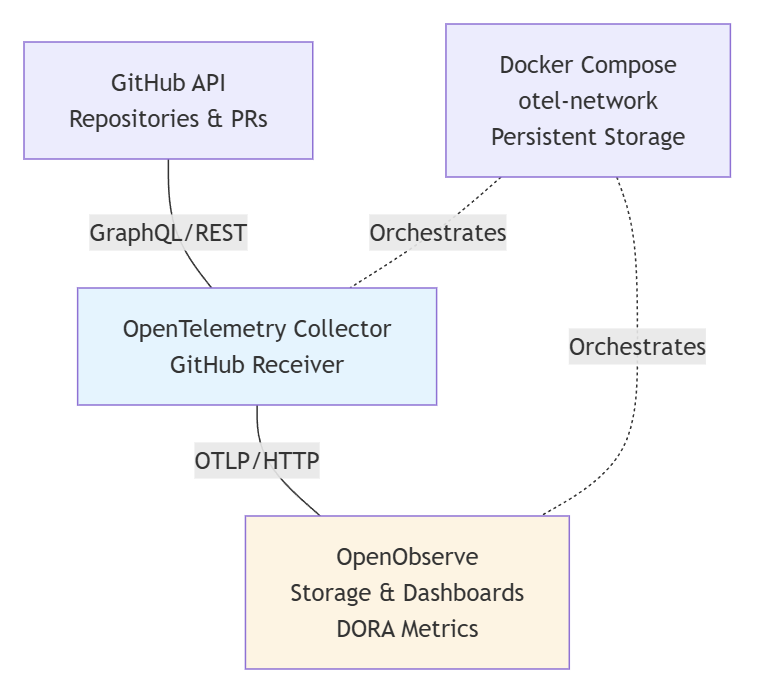
\includegraphics[width=0.7\textwidth]{system-architecture.png}
	\caption{System Architecture Overview}
	\label{fig:architecture}
\end{figure}

\textbf{OpenTelemetry Collector} (otelcol-contrib) scrapes
GitHub repositories every 60 seconds using the GitHub receiver.
Authentication uses a developer's Personal Access Token (PAT) via bearer token extension.
The collector exports metrics to OpenObserve via OTLP HTTP protocol.

\textbf{OpenObserve} stores time-series metrics and provides SQL-based querying for dashboard visualization.
Deployed on port 5080, it receives OTLP data at \texttt{/api/default/} endpoint.

\textbf{Docker Networking} connects both services via bridge network (\texttt{otel-network}) with persistent storage (\texttt{openobserve-data} volume) for metric retention.

The GitHub receiver supports flexible search queries (e.g., \texttt{org:<ORG>},
\texttt{is:private}, \texttt{is:pr is:open}) enabling targeted collection across
repositories and pull request states.


\section{Related Work}

\subsection{DORA Metrics Framework}

Forsgren, Humble, and Kim \cite{forsgren2018accelerate} established four metrics
that distinguish high-performing software teams based on multi-year research across thousands of organizations:

\begin{itemize}
	\item \textbf{Deployment Frequency}: Release cadence to production
	\item \textbf{Lead Time for Changes}: Duration from commit to production deployment
	\item \textbf{Change Failure Rate}: Percentage of deployments causing production failures
	\item \textbf{Time to Restore Service}: Recovery time from production incidents
\end{itemize}

Their research demonstrated strong correlations between these metrics and
organizational outcomes including profitability, productivity, and market share.

\subsection{Automated Metrics Collection}

OpenTelemetry \cite{opentelemetry2021} provides vendor-neutral observability
instrumentation.
The GitHub receiver \cite{opentelemetry-github-receiver}, currently at alpha stability, scrapes VCS
metrics via GitHub's GraphQL and REST APIs.
Kalliamvakou et al.
\cite{kalliamvakou2014promises} demonstrated the feasibility of deriving
development process metrics from version control systems, though they identified
challenges in data completeness and interpretation.

This project leverages the OpenTelemetry GitHub receiver to collect VCS metrics
aligned with OpenTelemetry semantic conventions v1.37.0, ensuring standardized
telemetry representation across platforms.

\section{Preliminary Data}

\subsection{Collected Metrics}

The GitHub receiver collects nine default metrics organized by their corresponding DORA metrics, as shown in Table \ref{tab:metrics}.
The GitHub reciever also collects telemetry attributes that provide dimensional and resource context for
filtering and aggregating metrics across repositories, organizations, and change states.
All metrics conform to OpenTelemetry semantic conventions v1.37.0 for VCS telemetry.


Change failure rate and time to restore service metrics have not yet been captured. Change failure rate
requires GitHub Actions workflow status or incident issue correlation. Time to restore service requires access to
deployment metrics from a production kubernetes cluster, which may not be feasible for this project.

\textbf{Metrics Not Yet Captured:}
\begin{itemize}
	\item \textbf{Change Failure Rate}:
	\item \textbf{Time to Restore Service}:
\end{itemize}

\begin{table}[htbp]
	\centering
	\caption{GitHub Receiver Metrics}
	\label{tab:metrics}
	\small
	\begin{tabular}{|p{6cm}|p{9cm}|}
		\hline
		\textbf{Metric Name}                   & \textbf{Description}                            \\
		\hline
		\multicolumn{2}{|c|}{\textit{Deployment Frequency Support}}                              \\
		\hline
		\texttt{vcs.change.count}              & Pull request counts by state (open/merged)      \\
		\hline
		\texttt{vcs.repository.count}          & Total repositories monitored                    \\
		\hline
		\multicolumn{2}{|c|}{\textit{Lead Time for Changes Support}}                             \\
		\hline
		\texttt{vcs.change.time\_to\_merge}    & Duration from PR creation to merge (seconds)    \\
		\hline
		\texttt{vcs.change.time\_to\_approval} & Duration from PR creation to approval (seconds) \\
		\hline
		\texttt{vcs.change.duration}           & Time PRs remain in open state (seconds)         \\
		\hline
		\multicolumn{2}{|c|}{\textit{Development Velocity Indicators}}                           \\
		\hline
		\texttt{vcs.ref.count}                 & Branch/tag counts per repository                \\
		\hline
		\texttt{vcs.ref.time}                  & Branch lifespan from creation (seconds)         \\
		\hline
		\texttt{vcs.ref.lines\_delta}          & Code churn (lines added/removed) vs. trunk      \\
		\hline
		\texttt{vcs.ref.revisions\_delta}      & Commit count ahead/behind trunk                 \\
		\hline
		\multicolumn{2}{|c|}{\textit{Telemetry Attributes}}                                      \\
		\hline
		\texttt{vcs.repository.name}           & Repository identifier                           \\
		\hline
		\texttt{vcs.repository.url.full}       & Complete repository URL                         \\
		\hline
		\texttt{vcs.change.state}              & PR state (open, merged)                         \\
		\hline
		\texttt{vcs.ref.type}                  & Reference type (branch, tag)                    \\
		\hline
		\texttt{vcs.ref.head.name}             & Branch name                                     \\
		\hline
		\multicolumn{2}{|c|}{\textit{Resource Attributes}}                                       \\
		\hline
		\texttt{vcs.provider.name}             & VCS provider (GitHub)                           \\
		\hline
		\texttt{vcs.owner.name}                & Organization/user account                       \\
		\hline
	\end{tabular}
\end{table}

\subsection{Visualization and Analysis}

OpenObserve dashboards visualize collected metrics through six panels:

\begin{figure}[htbp]
	\centering
	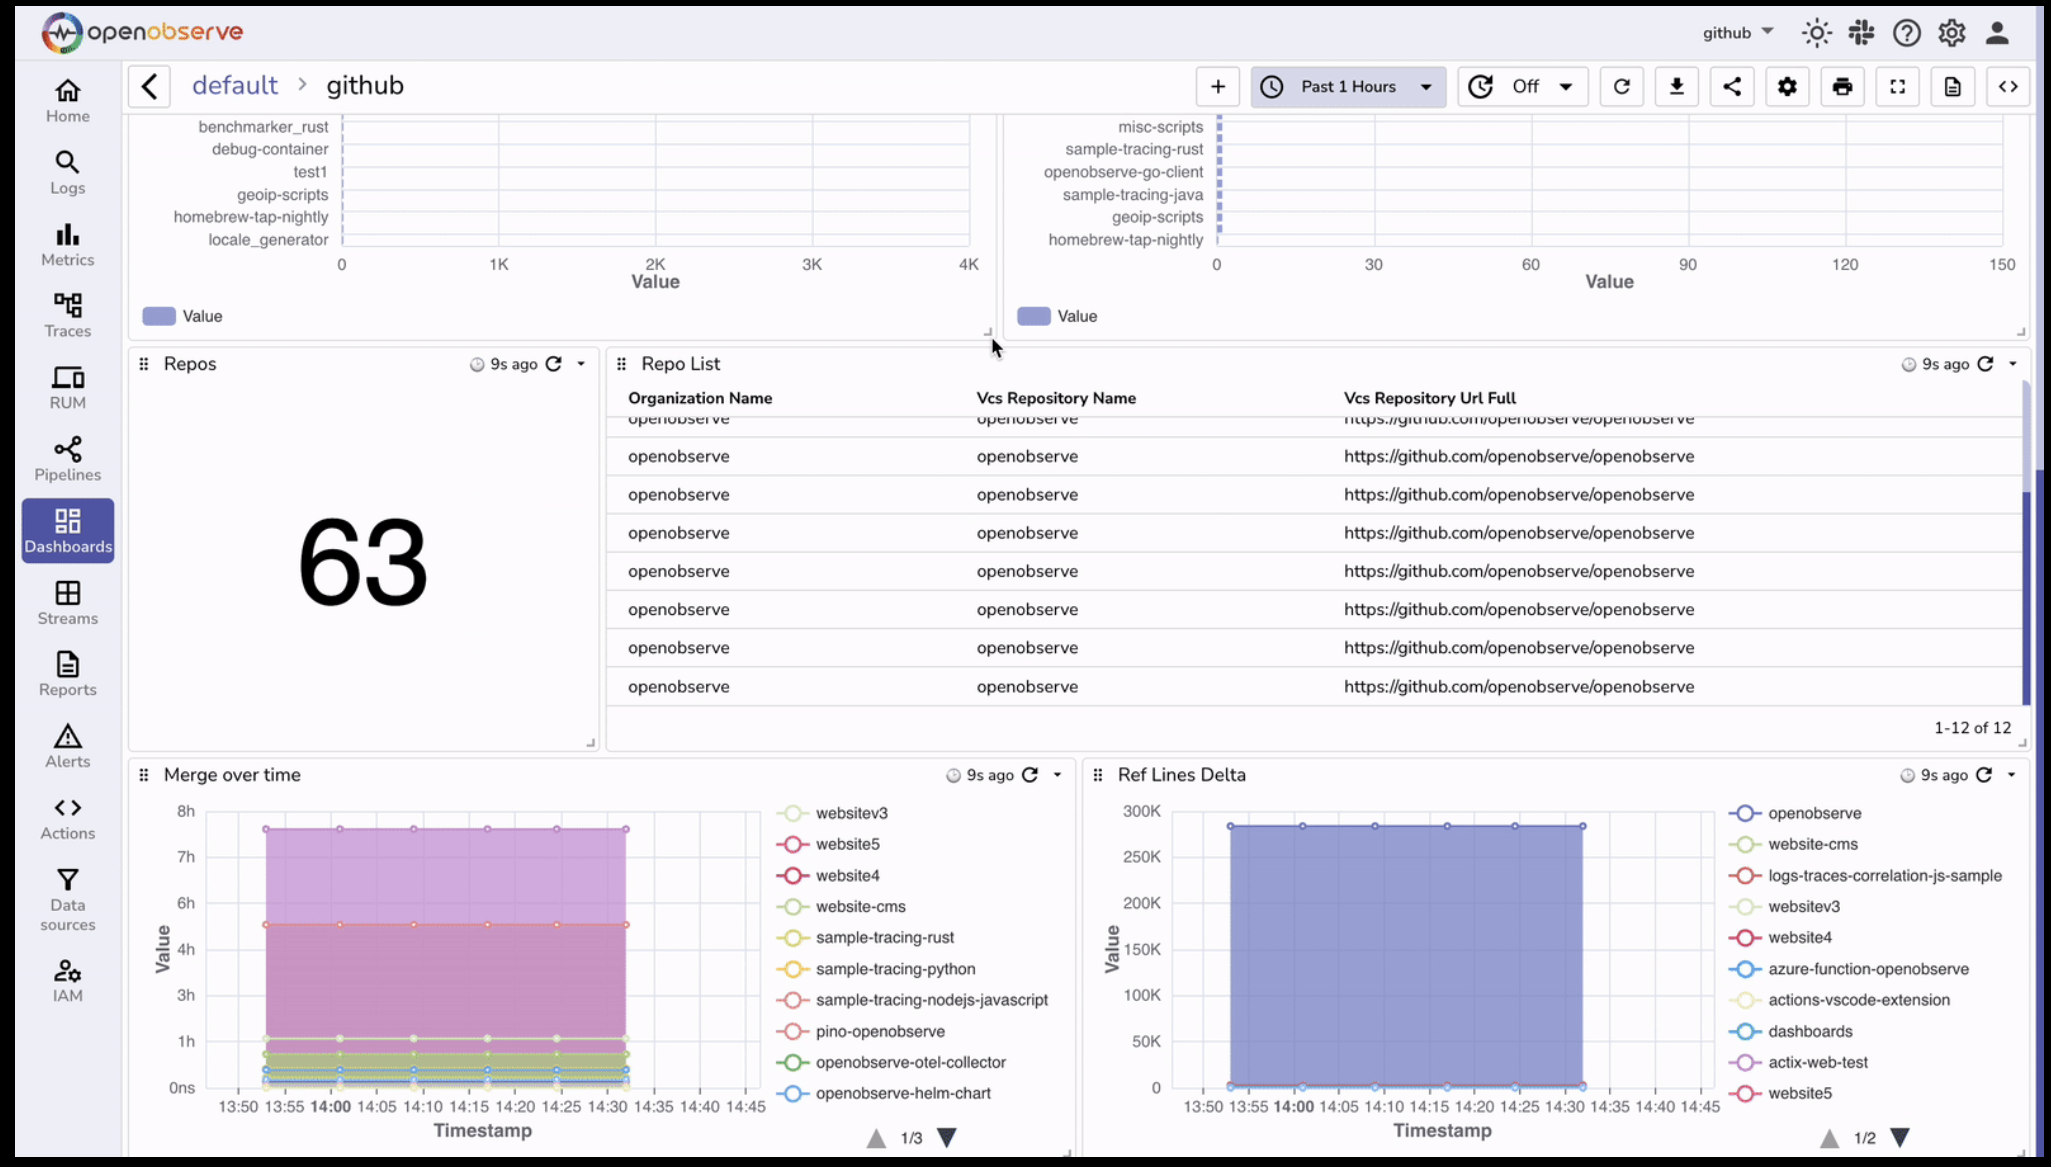
\includegraphics[width=0.7\textwidth]{openobserve-dashboard.png}
	\caption{OpenObserve Dashboard Visualizing GitHub Metrics}
	\label{fig:dashboard}
\end{figure}

\textbf{Repository Activity:}
\begin{itemize}
	\item Repository count (p95 aggregation)
	\item Top 10 repositories by change volume (horizontal bar chart)
	\item Reference (branch/tag) count by repository
	\item Repository list with organization and URL
\end{itemize}

\textbf{DORA-Aligned Time Series:}
\begin{itemize}
	\item Merge time trends over time (p95, millisecond precision, repository breakdown)
	\item Code churn (lines delta) trends over time (repository breakdown)
\end{itemize}

SQL queries employ 95th percentile aggregation to filter outliers and
histogram-based temporal bucketing for trend analysis.


\bibliographystyle{IEEEtran}
\bibliography{references}

\end{document}
